\documentclass{article}

\PassOptionsToPackage{table,svgnames}{xcolor}\usepackage{graphicx}
\usepackage{tikz-network}
\usepackage{xcolor}

\begin{document}
\begin{titlepage}
    \centering
    % Logo
    
\includegraphics[width=0.6\textwidth]{logo-tec.png}\par\vspace{1cm}

    % University and course
    {\large Escuela de Ingenier\'ia en Computaci\'on\par}
    {\large Investigaci\'on de Operaciones\par}
    \vspace{2cm}

    % Title
    {\Large Rutas \'Optimas\par}
    {\large Algoritmo de Floyd\par}
    \vspace{2cm}

    % Group and professor
    {\large Grupo 40\par}
    {\large Profesor: Francisco Torres Rojas\par}
    \vspace{3cm}

    % Student info
    {\large Carmen Hidalgo Paz\par}
    {\large Carn\'e: 2020030538\par}
    \vspace{1cm}
    {\large Melissa Carvajal Charpentier\par}
    {\large Carn\'e: 2022197088\par}
    \vspace{1cm}
    {\large Josu\'e Soto Gonz\'alez\par}
    {\large Carn\'e: 2023207915\par}
    \vspace{1cm}

    % Date
    {\large 12 de Septiembre del 2025\par}
\end{titlepage}
\definecolor{KirbyPink}{HTML}{D74894}
\definecolor{LightPink}{HTML}{FFBFBF}

\newpage


\section{Floyd's Algorithm}
This program consists of Floyd's algorithm to obtain the shortest path between any pair of nodes in a graph with weighted distances.
Floyd's algorithm compares the distance between any two given nodes and by passing through another city in between, if the result is less than the original then it chooses the shortest one. After contemplating all nodes in the graph, the graph is guaranteed to have all the shortest distances between any two nodes in the graph. These changes are recorded in another matrix called P that helps determine the shortest path between any two nodes.
\section{Robert W. Floyd (1936–2001)}
\begin{center}
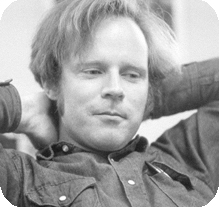
\includegraphics[width=0.25\textwidth]{floyd.jpg}
\end{center}
Robert Willoughby Floyd was a computer scientist that lived from 1936 to 2001. He made great advances in computer science and developed an algorithm to find the shortest paths between any two nodes for a directed graph. He was awarded a Turing Award in 1978.


\section{Initial Graph}
\begin{center}
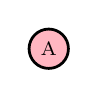
\begin{tikzpicture}
 \Vertex[x=5.000000, y=0.000000, color=LightPink, size=0.5, label={A}]{A}
\end{tikzpicture}
\end{center}
\section{Table $D_{0}$}
\begin{center}
    \begin{tabular}{|c||c|}
        \hline
        \textbf{D} & \textbf{A} \\
        \hline
        \hline
        \textbf{A}& 0 \\
        \hline
    \end{tabular}
\end{center}


\section{Table $P_{0}$}
\begin{center}
    \begin{tabular}{|c||c|}
        \hline
        \textbf{P} & \textbf{A} \\
        \hline
        \hline
        \textbf{A}& 0 \\
        \hline
    \end{tabular}
\end{center}


\section{Table $D_{1}$}
\begin{center}
    \begin{tabular}{|c||c|}
        \hline
        \textbf{D} & \textbf{A} \\
        \hline
        \hline
        \textbf{A}& 0 \\
        \hline
    \end{tabular}
\end{center}


\section{Table $P_{1}$}
\begin{center}
    \begin{tabular}{|c||c|}
        \hline
        \textbf{P} & \textbf{A} \\
        \hline
        \hline
        \textbf{A}& 0 \\
        \hline
    \end{tabular}
\end{center}


\section*{Current city: New York}
\begin{center}
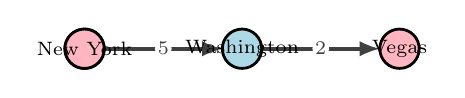
\begin{tikzpicture}
<<<<<<< HEAD
 \Vertex[x=0, y=0, color=LightPink, size=0.5, label={A}]{A}
=======
 \Vertex[x=0, y=0, color=LightPink, size=0.5, label={New York}]{A}
 \Vertex[x=2, y=0, color=LightBlue, size=0.5, label={Washington}]{E}
 \Edge[label=$5$, Direct](A)(E)
 \Vertex[x=4, y=0, color=LightPink, size=0.5, label={Vegas}]{B}
 \Edge[label=$2$, Direct](E)(B)
\end{tikzpicture}
\end{center}
\begin{center}
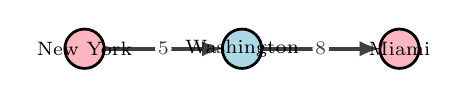
\begin{tikzpicture}
 \Vertex[x=0, y=0, color=LightPink, size=0.5, label={New York}]{A}
 \Vertex[x=2, y=0, color=LightBlue, size=0.5, label={Washington}]{E}
 \Edge[label=$5$, Direct](A)(E)
 \Vertex[x=4, y=0, color=LightPink, size=0.5, label={Miami}]{C}
 \Edge[label=$8$, Direct](E)(C)
\end{tikzpicture}
\end{center}
\begin{center}
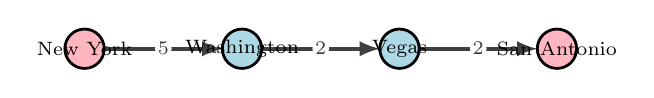
\begin{tikzpicture}
 \Vertex[x=0, y=0, color=LightPink, size=0.5, label={New York}]{A}
 \Vertex[x=2, y=0, color=LightBlue, size=0.5, label={Washington}]{E}
 \Edge[label=$5$, Direct](A)(E)
 \Vertex[x=4, y=0, color=LightBlue, size=0.5, label={Vegas}]{B}
 \Edge[label=$2$, Direct](E)(B)
 \Vertex[x=6, y=0, color=LightPink, size=0.5, label={San Antonio}]{D}
 \Edge[label=$2$, Direct](B)(D)
\end{tikzpicture}
\end{center}
\begin{center}
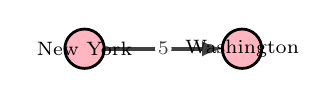
\begin{tikzpicture}
 \Vertex[x=0, y=0, color=LightPink, size=0.5, label={New York}]{A}
 \Vertex[x=2, y=0, color=LightPink, size=0.5, label={Washington}]{E}
 \Edge[label=$5$, Direct](A)(E)
\end{tikzpicture}
\end{center}
\section*{Current city: Vegas}
\begin{center}
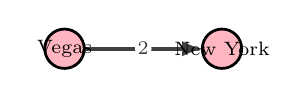
\begin{tikzpicture}
 \Vertex[x=0, y=0, color=LightPink, size=0.5, label={Vegas}]{B}
 \Vertex[x=2, y=0, color=LightPink, size=0.5, label={New York}]{A}
 \Edge[label=$2$, Direct](B)(A)
\end{tikzpicture}
\end{center}
\begin{center}
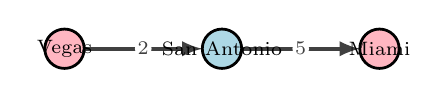
\begin{tikzpicture}
 \Vertex[x=0, y=0, color=LightPink, size=0.5, label={Vegas}]{B}
 \Vertex[x=2, y=0, color=LightBlue, size=0.5, label={San Antonio}]{D}
 \Edge[label=$2$, Direct](B)(D)
 \Vertex[x=4, y=0, color=LightPink, size=0.5, label={Miami}]{C}
 \Edge[label=$5$, Direct](D)(C)
\end{tikzpicture}
\end{center}
\begin{center}
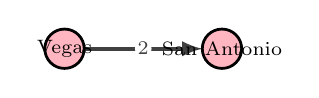
\begin{tikzpicture}
 \Vertex[x=0, y=0, color=LightPink, size=0.5, label={Vegas}]{B}
 \Vertex[x=2, y=0, color=LightPink, size=0.5, label={San Antonio}]{D}
 \Edge[label=$2$, Direct](B)(D)
\end{tikzpicture}
\end{center}
\begin{center}
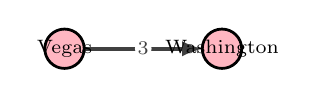
\begin{tikzpicture}
 \Vertex[x=0, y=0, color=LightPink, size=0.5, label={Vegas}]{B}
 \Vertex[x=2, y=0, color=LightPink, size=0.5, label={Washington}]{E}
 \Edge[label=$3$, Direct](B)(E)
\end{tikzpicture}
\end{center}
\section*{Current city: Miami}
\begin{center}
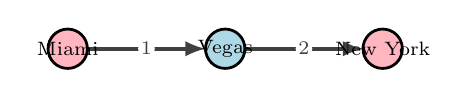
\begin{tikzpicture}
 \Vertex[x=0, y=0, color=LightPink, size=0.5, label={Miami}]{C}
 \Vertex[x=2, y=0, color=LightBlue, size=0.5, label={Vegas}]{B}
 \Edge[label=$1$, Direct](C)(B)
 \Vertex[x=4, y=0, color=LightPink, size=0.5, label={New York}]{A}
 \Edge[label=$2$, Direct](B)(A)
\end{tikzpicture}
\end{center}
\begin{center}
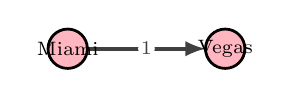
\begin{tikzpicture}
 \Vertex[x=0, y=0, color=LightPink, size=0.5, label={Miami}]{C}
 \Vertex[x=2, y=0, color=LightPink, size=0.5, label={Vegas}]{B}
 \Edge[label=$1$, Direct](C)(B)
\end{tikzpicture}
\end{center}
\begin{center}
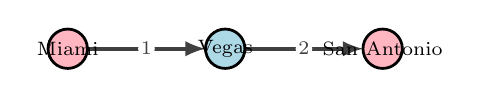
\begin{tikzpicture}
 \Vertex[x=0, y=0, color=LightPink, size=0.5, label={Miami}]{C}
 \Vertex[x=2, y=0, color=LightBlue, size=0.5, label={Vegas}]{B}
 \Edge[label=$1$, Direct](C)(B)
 \Vertex[x=4, y=0, color=LightPink, size=0.5, label={San Antonio}]{D}
 \Edge[label=$2$, Direct](B)(D)
\end{tikzpicture}
\end{center}
\begin{center}
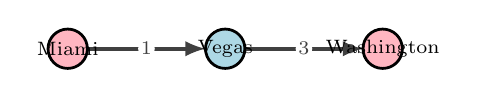
\begin{tikzpicture}
 \Vertex[x=0, y=0, color=LightPink, size=0.5, label={Miami}]{C}
 \Vertex[x=2, y=0, color=LightBlue, size=0.5, label={Vegas}]{B}
 \Edge[label=$1$, Direct](C)(B)
 \Vertex[x=4, y=0, color=LightPink, size=0.5, label={Washington}]{E}
 \Edge[label=$3$, Direct](B)(E)
\end{tikzpicture}
\end{center}
\section*{Current city: San Antonio}
\begin{center}
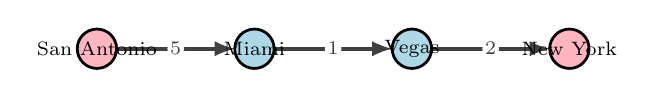
\begin{tikzpicture}
 \Vertex[x=0, y=0, color=LightPink, size=0.5, label={San Antonio}]{D}
 \Vertex[x=2, y=0, color=LightBlue, size=0.5, label={Miami}]{C}
 \Edge[label=$5$, Direct](D)(C)
 \Vertex[x=4, y=0, color=LightBlue, size=0.5, label={Vegas}]{B}
 \Edge[label=$1$, Direct](C)(B)
 \Vertex[x=6, y=0, color=LightPink, size=0.5, label={New York}]{A}
 \Edge[label=$2$, Direct](B)(A)
\end{tikzpicture}
\end{center}
\begin{center}
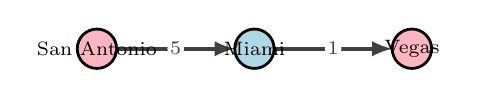
\begin{tikzpicture}
 \Vertex[x=0, y=0, color=LightPink, size=0.5, label={San Antonio}]{D}
 \Vertex[x=2, y=0, color=LightBlue, size=0.5, label={Miami}]{C}
 \Edge[label=$5$, Direct](D)(C)
 \Vertex[x=4, y=0, color=LightPink, size=0.5, label={Vegas}]{B}
 \Edge[label=$1$, Direct](C)(B)
\end{tikzpicture}
\end{center}
\begin{center}
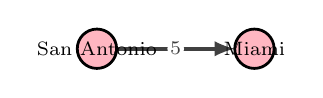
\begin{tikzpicture}
 \Vertex[x=0, y=0, color=LightPink, size=0.5, label={San Antonio}]{D}
 \Vertex[x=2, y=0, color=LightPink, size=0.5, label={Miami}]{C}
 \Edge[label=$5$, Direct](D)(C)
\end{tikzpicture}
\end{center}
\begin{center}
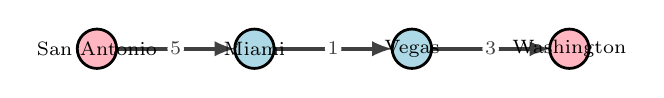
\begin{tikzpicture}
 \Vertex[x=0, y=0, color=LightPink, size=0.5, label={San Antonio}]{D}
 \Vertex[x=2, y=0, color=LightBlue, size=0.5, label={Miami}]{C}
 \Edge[label=$5$, Direct](D)(C)
 \Vertex[x=4, y=0, color=LightBlue, size=0.5, label={Vegas}]{B}
 \Edge[label=$1$, Direct](C)(B)
 \Vertex[x=6, y=0, color=LightPink, size=0.5, label={Washington}]{E}
 \Edge[label=$3$, Direct](B)(E)
\end{tikzpicture}
\end{center}
\section*{Current city: Washington}
\begin{center}
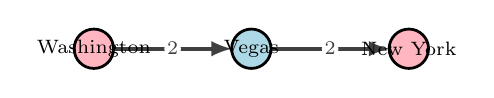
\begin{tikzpicture}
 \Vertex[x=0, y=0, color=LightPink, size=0.5, label={Washington}]{E}
 \Vertex[x=2, y=0, color=LightBlue, size=0.5, label={Vegas}]{B}
 \Edge[label=$2$, Direct](E)(B)
 \Vertex[x=4, y=0, color=LightPink, size=0.5, label={New York}]{A}
 \Edge[label=$2$, Direct](B)(A)
\end{tikzpicture}
\end{center}
\begin{center}
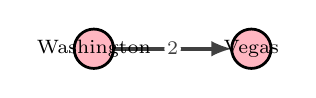
\begin{tikzpicture}
 \Vertex[x=0, y=0, color=LightPink, size=0.5, label={Washington}]{E}
 \Vertex[x=2, y=0, color=LightPink, size=0.5, label={Vegas}]{B}
 \Edge[label=$2$, Direct](E)(B)
\end{tikzpicture}
\end{center}
\begin{center}
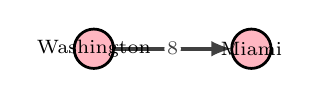
\begin{tikzpicture}
 \Vertex[x=0, y=0, color=LightPink, size=0.5, label={Washington}]{E}
 \Vertex[x=2, y=0, color=LightPink, size=0.5, label={Miami}]{C}
 \Edge[label=$8$, Direct](E)(C)
\end{tikzpicture}
\end{center}
\begin{center}
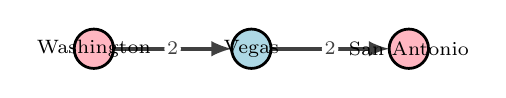
\begin{tikzpicture}
 \Vertex[x=0, y=0, color=LightPink, size=0.5, label={Washington}]{E}
 \Vertex[x=2, y=0, color=LightBlue, size=0.5, label={Vegas}]{B}
 \Edge[label=$2$, Direct](E)(B)
 \Vertex[x=4, y=0, color=LightPink, size=0.5, label={San Antonio}]{D}
 \Edge[label=$2$, Direct](B)(D)
>>>>>>> origin/main
\end{tikzpicture}
\end{center}
\end{document}
